\chapter{Analisis}
\label{chap:analisis}
Pada bab ini dijelaskan mengenai analisis Google VR SDK, \textit{Google StreetView API}, \textit{Google Directions API}, dan  sensor \textit{step detector}, juga cara memanfaatkan   mengintegrasikan semua komponen tersebut secara bertahap untuk membentuk aplikasi \textit{jogging} virtual. 

\section{Masalah yang akan Diselesaikan}
Ada tiga hal yang harus diperhatikan untuk membangun \textit{virtual jogging app}, yaitu pemandangan, rute perjalanan, dan perubahan pemandangan sesuai dengan rute perjalanan. Pemandangan dapat diciptakan dengan menggunakan Google VR SDK dan \textit{Google StreetView API}, rute perjalanan dari pelari dapat diperoleh menggunakan \textit{Google Directions API}, dan perubahan dari pemandangan diatur dengan sensor gerak. 

\section{Analisis Google VR SDK}
Dari aplikasi HelloVR yang disedikaan di Google VR SDK, ada beberapa kebutuhan yang dapat dipelajari, terutama dari \textit{folder assets}. \textit{Folder assets} berisi bangun ruang tiga dimensi dari ruangan dan objek-objek beserta tekstur masing-masing ruangan dan objek~\cite{quickstart-google-vr}. \textit{Folder assets} berisi \textit{file-file} OBJ seperti CubeRoom.obj, Icosahedron.obj, QuadSphere.obj, dan TriSphere.obj. CubeRoom.obj berfungsi sebagai ruang dalam dunia VR itu, sementara \textit{file-file} OBJ lain adalah objek-objek yang ada di dalam dunia aplikasi HelloVR. Masing-masing \textit{file-file} OBJ dipasangkan dengan \textit{file-file} PNG yang adalah tekstur-tekstur masing-masing \textit{file-file} OBJ. Dari analisis \textit{folder assets} aplikasi HelloVR, dibutuhkan dunia VR yang terdefinisi dengan tampilan seperti di dunia nyata. Dunia VR ini dapat dibentuk lewat dua komponen utama: bangun ruang tiga dimensi dan gambar dari \textit{Google StreetView API}. Bangun ruang tiga dimensi berfungsi sebagai batasan dunia VR tersebut, sementara gambar \textit{Google StreetView API} memberi pemandangan dari tempat dunia nyata. Dengan menciptakan bangun ruang tiga dimensi yang ditambahkan tekstur gambar \textit{Google StreetView API}, pemandangan seperti di dunia nyata dapat direalisasikan pada aplikasi VR. 

Agar dapat membuat pemandangan VR seperti dunia nyata yang bergerak, tekstur dari bangun ruang tiga dimensi yang sudah diciptakan harus berubah-ubah. Perubahan dari tekstur yang diperoleh \textit{Google StreetView API} haruslah sesuai dengan rute perjalanan. \textit{Google Directions API}lah yang dapat digunakan untuk menentukan rute perjalanan dari asal dan tujuan yang dapat digunakan untuk perubahan gambar tekstur untuk bangun ruang tiga dimensi. 

Komponen terakhir dari aplikasi \textit{jogging} virtual yang harus dimanfaatkan adalah sensor \textit{step detector}. Sensor \textit{step detector} ini digunakan untuk menentukan ritme perubahan dari tekstur bangun ruang tiga dimensi. Saat langkah kaki dari pengguna terdeteksi, barulah gambar tekstur dari bangun ruang tiga dimensi diubah seturut rute perjalanan dari \textit{Google Directions API}.

\section{Analisis Pembuatan Bangun Ruang Tiga Dimensi}

Bangun ruang tiga dimensi yang tepat untuk dibuat adalah silinder atau tabung. Alasan dipilihnya bentuk silinder ini adalah bentuk silinder cukup merepresentasikan pandangan lateral atau samping dari manusia di dunia nyata. Permukaan samping inilah yang nantinya akan diisi tekstur dari gambar \textit{Google StreetView API}. 

Untuk membuat dunia berbentuk silinder, kakas yang digunakan adalah \textit{Blender} versi 2.81. Gambar menunjukkan tampilan \textit{UI} \textit{Blender} versi 2.81. Setelah bangun ruang silinder dibentuk dari kakas \textit{Blender}, bangun ruang itu disimpan dalam sebuah \textit{file} OBJ. 

\begin{figure}[h]
	\centering
		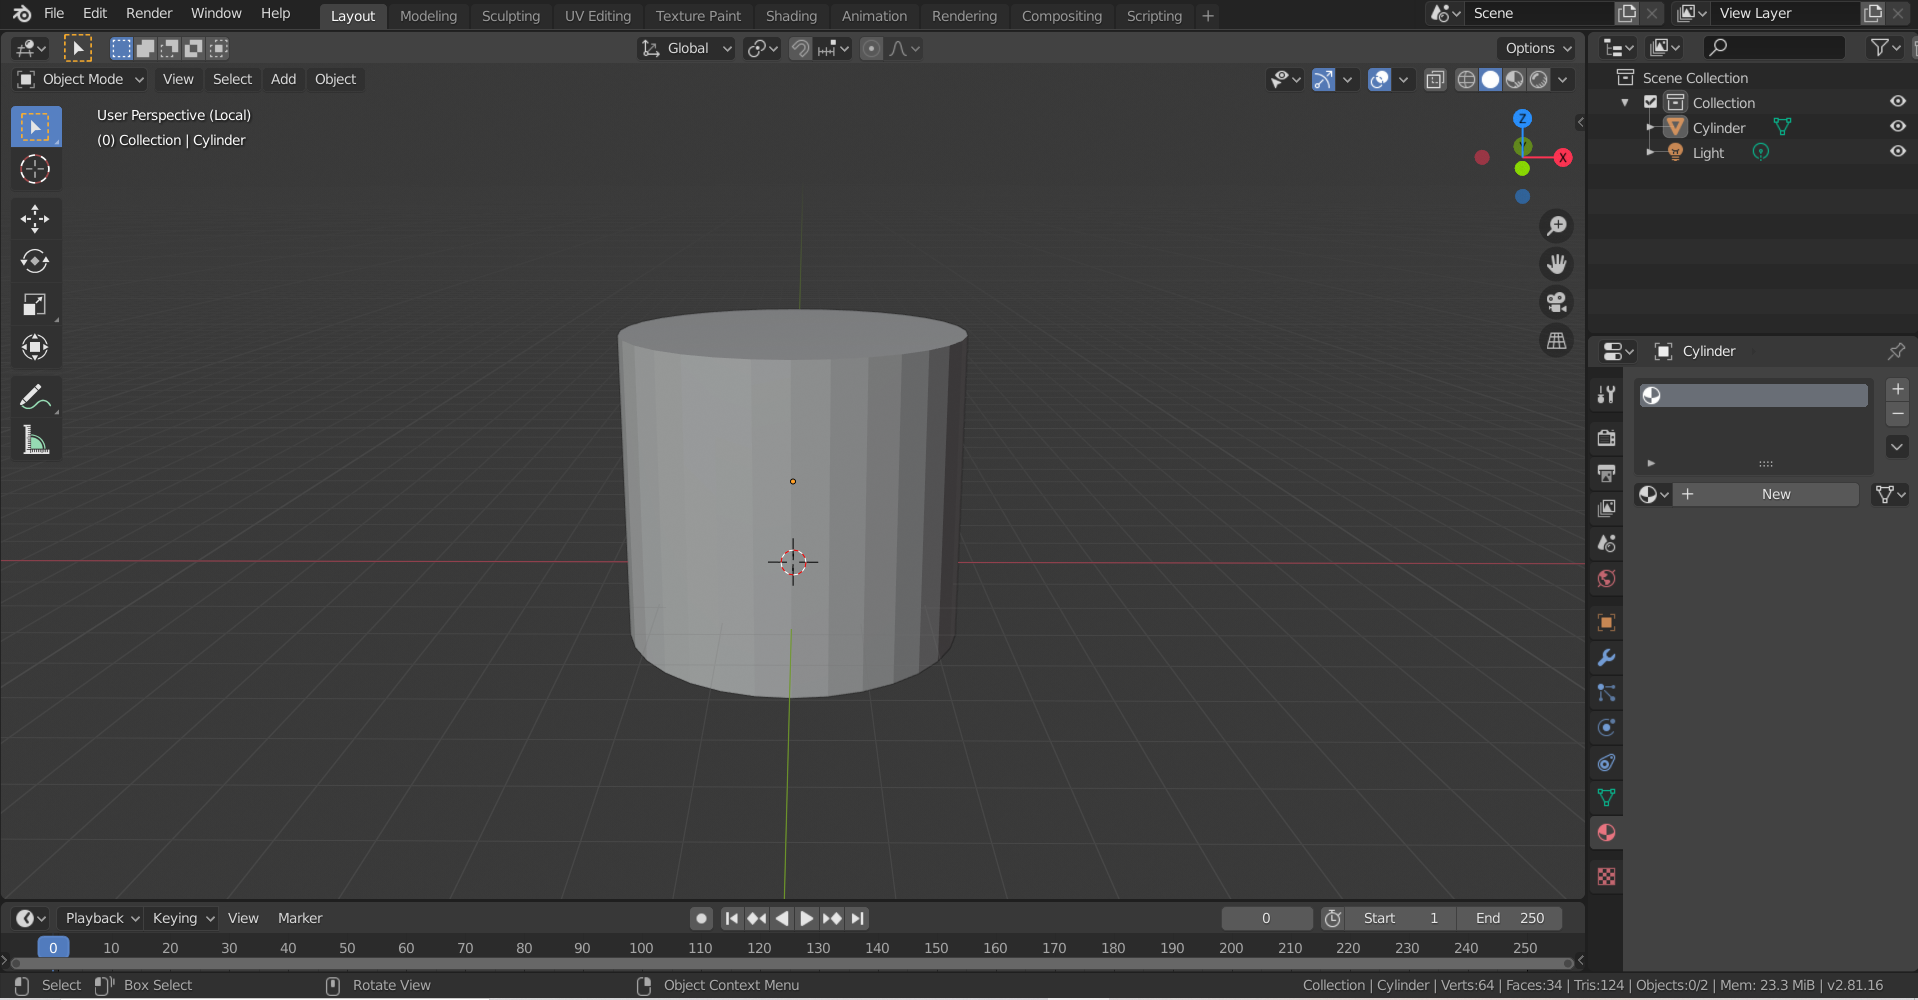
\includegraphics[scale=0.4]{Gambar/blender.png}
	\caption{Tampilan \textit{UI Blender} Blender versi 2.81}
	\label{fig:blender-ui}
\end{figure}

\section{Menampilkan Gambar \textit{StreetView API} pada Bangun Ruang Silinder}
Untuk membuat tampilan dunia VR yang sempurna, bagian kedua yang harus dipenuhi adalah pemandangan yang dihasilkan lewat gambar \textit{Google StreetView API} di permukaan samping silinder. 
\textit{Google StreetView API} menghasilkan gambar pemandangan dari satu arah pandang, maka haruslah dikumpulkan gambar-gambar dari arah-arah yang lain untuk membentuk pemandangan sekeliling yang sempurna dan terlihat seperti dunia nyata~\cite{streetview-api}. Sebagai contoh, gambar dari empat arah (utara, selatan, timur, dan barat) harus digabungkan untuk menghasilkan pemandangan seperti  dunia nyata. Hal yang harus dilakukan untuk mencapai hal tersebut adalah menggabungkan gambar-gambar dari atribut \textit{heading} dari empat arah, dengan satu arah yang berlawanan dengan arah yang lain, lalu dua arah lain yang tegak lurus dengan arah pertama. Dengan kata lain, selisih setiap dua nilai \textit{heading} yang berurutan  bernilai 90 (misalnya \textit{heading} dengan nilai 0, 90, 180 dan 270). Gambar \ref{fig:comp-streetview} memperlihatkan empat gambar berukuran $600\times300$ \textit{StreetView} dengan berbagai macam \textit{StreetView} dengan syarat tersebut.

\begin{figure}[]
	\begin{subfigure}{.5\textwidth}
  		\centering
  		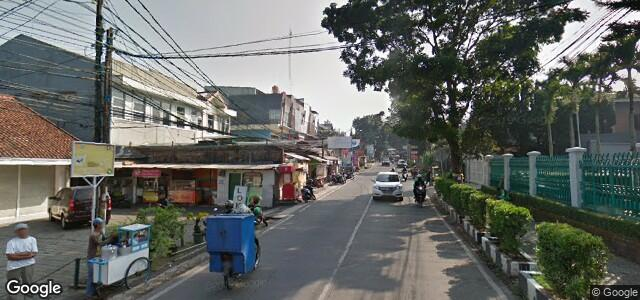
\includegraphics[width=1\linewidth]{Gambar/streetview0.png}
  		\caption{\textit{heading}=0}
  		\label{fig:streetview0}
	\end{subfigure}
	\begin{subfigure}{.5\textwidth}
  		\centering
  		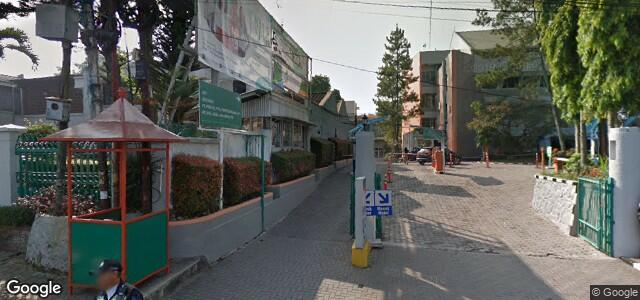
\includegraphics[width=1\linewidth]{Gambar/streetview90.png}
  		\caption{\textit{heading}=90}
  		\label{fig:streetview90}
	\end{subfigure}
	\begin{subfigure}{.5\textwidth}
  		\centering
  		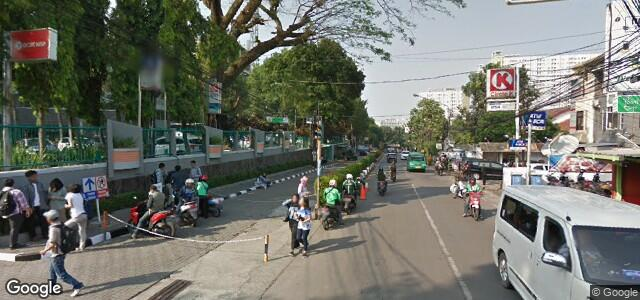
\includegraphics[width=1\linewidth]{Gambar/streetview180.png}
  		\caption{\textit{heading}=180}
  		\label{fig:streetview180}
	\end{subfigure}
	\begin{subfigure}{.5\textwidth}
  		\centering
  		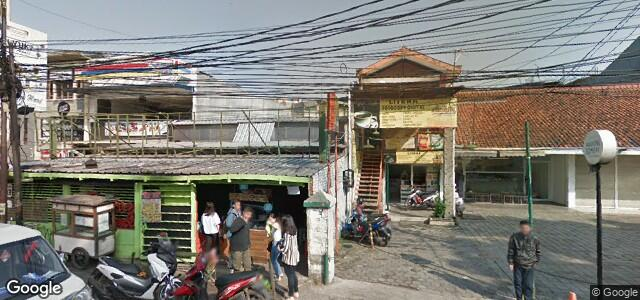
\includegraphics[width=1\linewidth]{Gambar/streetview270.png}
  		\caption{\textit{heading}=270}
  		\label{fig:streetview270}
	\end{subfigure}
	\caption{Gambar dari \textit{StreetView API} berukuran $600\times300$  dengan parameter \textit{heading} yang berbeda-beda}
\label{fig:comp-streetview}
\end{figure}

Setelah mendapatkan gambar \textit{StreetView} dari semua arah, gambar-gagmbar tersebut digabungkan sehingga membentuk pemandangan seperti ada di lokasi tersebut. Gambar \ref{fig:streetview-vr} menunjukkan hasil penggabungan empat gambar dengan deskripsi di atas.

\begin{figure}[h]
	\centering
		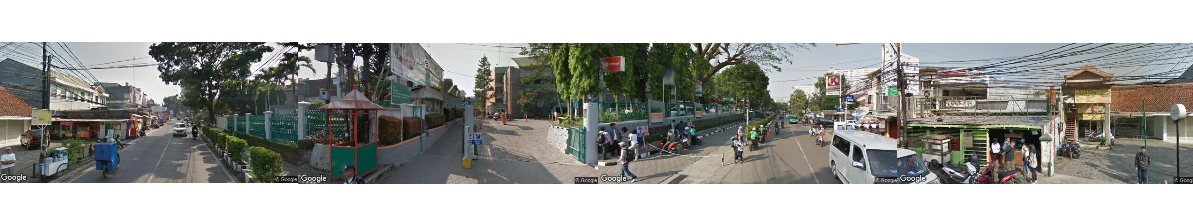
\includegraphics[width=6.5in,height=3in]{Gambar/connected_streetview.png}
	\caption{Contoh hasil penggabungan empat gambar \textit{StreetView}}
	\label{fig:streetview-vr}
\end{figure}

Setelah mendapatkan gambar \textit{StreetView} yang sudah digabungkan tersebut, gambar tersebut dapat dimanfaatkan sebagai tekstur untuk ruang pada \textit{file} OBJ yang berbentuk silinder sehingga pemandangan \textit{StreetView} dapat ditampilkan pada dunia VR. Gambar tersebut dapat di-\textit{bind} dengan bangun ruang silinder yang akan dibuat.

\section{Analisis \textit{Google Directions API}}
Untuk mendapatkan rute perjalanan, \textit{Directions API} dapat dimanfaatkan~\cite{directions-api}. \textit{File} yang diperoleh lewat \textit{Directions API} adalah \textit{file} JSON yang memiliki \textit{key} dan \textit{value}. Ada beberapa atribut (\textit{key}) dengan nilai (\textit{value}) yang ada pada \textit{file} JSON dari hasil pemanggilan \textit{Directions API} yang dapat dimanfaatkan.

\subsection{Menentukan Atribut yang akan Digunakan dari JSON \textit{Directions}}
\textit{File} JSON yang dihasilkan memiliki beberapa tingkat \textit{key} dan \textit{value}. Pada tingkat pertama, ada tiga \textit{key}: \textit{geocoded\_waypoints}, \textit{status} dan \textit{routes}. \textit{Key} yang dapat digunakan adalah \textit{routes} yang menunjukkan jalan yang akan ditempuh. Pada tingkat berikutnya, \textit{key routes} memiliki \textit{value} seperti \textit{bounds}, \textit{copyrights}, dan \textit{legs}. Jika melihat bagian \textit{legs} yang menampung atribut-atribut jalan yang ditempuh, ada {\it distance}, {\it duration}, {\it end\_location}, {\it html\_instructions}, {\it maneuver}, {\it polyline}, {\it start\_location}, dan \textit{travel\_mode}. Dari beberapa atribut dari \textit{legs}, yang dapat digunakan adalah \textit{end\_location} dan \textit{start\_location}, yang menunjuk kepada posisi garis lintang dan garis bujur titik ujung dari jalan yang sedang ditempuh. 

\begin{lstlisting}[caption={Atribut \textit{legs} dari \textit{Directions API}},label={list:directions_legs},language=java]
         "legs" : [
            {
               "distance" : {
                  "text" : "3.0 km",
                  "value" : 2980
               },
               "duration" : {
                  "text" : "35 mins",
                  "value" : 2116
               },
               "end_address" : "Jl. Ir. H. Juanda No.100, Lebakgede...",
               "end_location" : {
                  "lat" : -6.893148,
                  "lng" : 107.6131791
               },
               "start_address" : "Jl. Ciumbuleuit No.94, Hegarmanah...",
               "start_location" : {
                  "lat" : -6.8746719,
                  "lng" : 107.6046127
               },
               "steps" : [
                  {
                     "distance" : {
                        "text" : "1.0 km",
                        "value" : 1008
                     },
                     "duration" : {
                        "text" : "11 mins",
                        "value" : 667
                     },
                     "end_location" : {
                        "lat" : -6.8833328,
                        "lng" : 107.6049108
                     },
                     "html_instructions" : "Head \u003cb\u003esouth...",
                     "polyline" : {
                        "points" : "tu}h@yowoSdAP|AL`Cb@dAHHBvC..."
                     },
                     "start_location" : {
                        "lat" : -6.8746719,
                        "lng" : 107.6046127
                     },
                     "travel_mode" : "WALKING"
                  },
                  {
                     "distance" : {
                        "text" : "1.1 km",
                        "value" : 1078
                     },
                     "duration" : {
                        "text" : "14 mins",
                        "value" : 834
                     },
                     "end_location" : {
                        "lat" : -6.885218399999999,
                        "lng" : 107.6137497
                     },
                     "html_instructions" : "Turn \u003cb\u003eleft\u003c/b...",
                     "maneuver" : "turn-left",
                     "polyline" : {
                        "points" : "xk_i@uqwoSCEAECKAM?K?E?..."
                     },
                     "start_location" : {
                        "lat" : -6.8833328,
                        "lng" : 107.6049108
                     },
                     "travel_mode" : "WALKING"
                  },
                  {
                     "distance" : {
                        "text" : "0.9 km",
                        "value" : 884
                     },
                     "duration" : {
                        "text" : "10 mins",
                        "value" : 603
                     },
                     "end_location" : {
                        "lat" : -6.893140799999999,
                        "lng" : 107.6130843
                     },
                     "html_instructions" : "Turn \u003cb\u003eright...",
                     "maneuver" : "turn-right",
                     "polyline" : {
                        "points" : "rw_i@}hyoSzCLlAHz@Bd@@fB@tBDfABR@L..."
                     },
                     "start_location" : {
                        "lat" : -6.885218399999999,
                        "lng" : 107.6137497
                     },
                     "travel_mode" : "WALKING"
                  },
                  {
                     "distance" : {
                        "text" : "10 m",
                        "value" : 10
                     },
                     "duration" : {
                        "text" : "1 min",
                        "value" : 12
                     },
                     "end_location" : {
                        "lat" : -6.893148,
                        "lng" : 107.6131791
                     },
                     "html_instructions" : "Turn \u003cb\u003eleft\u003c...",
                     "maneuver" : "turn-left",
                     "polyline" : {
                        "points" : "biai@wdyoS@S"
                     },
                     "start_location" : {
                        "lat" : -6.893140799999999,
                        "lng" : 107.6130843
                     },
                     "travel_mode" : "WALKING"
                  }
               ],
               "traffic_speed_entry" : [],
               "via_waypoint" : []
            }
         ],
         "overview_polyline" : {
            "points" : "tu}h@yowoSdAP|AL`Cb@dAH`Dd@~Bd@hG..."
         },
         "summary" : "Jl. Ciumbuleuit, Jl. Siliwangi...",
         "warnings" : [
            "Walking directions are in beta. Use caution..."
         ],
         "waypoint_order" : []
      }
   ],
   "status" : "OK"
}
\end{lstlisting}

Listing \ref{list:directions_legs} menunjukkan atribut \textit{legs} dari hasil JSON \textit{Directions}.



\subsection{Cara Memanfaatkan Atribut}
\label{subs:directions-attr-use}
Setelah memperoleh nilai \textit{end\_location} dan \textit{start\_location}, jalur tempuh pada jalan yang sedang ditempuh dapat ditentukan lewat posisi garis lintang dan garis bujur kedua titik ujung jalan. Cara untuk membentuk jalan secara matematis adalah menggunakan selisih antara garis lintang dan garis bujur satu titik ujung jalan ke titik ujung jalan lain. 

\section{Analisis \textit{Step Detector Sensor}}
Subbab ini akan menunjukkan hasil eksperimen pengujian \textit{step detector sensor} dan menjelaskan cara memanfaatkannya pada aplikasi. 

\subsection{Eksperimen Pengujian \textit{Step Detector Sensor}}
\textit{Step detector sensor} adalah sensor yang mendeteksi langkah kaki, lalu merangsang suatu aksi di dalam aplikasi. Oleh karena itu, eksperimen untuk melihat gerakan-gerakan yang membuat perangkat bergerak mendeteksi langkah kaki dilakukan. Metode melakukan eksperimen ini adalah dengan memilih beberapa jenis gerakan pada sumbu-sumbu sensor perangkat bergerak, lalu melihat gerakan mana saja yang mendapat rangsang untuk memicu aksi pada aplikasi. Gambar \ref{fig:axis-device} menunjukkan sumbu-sumbu yang dibaca sensor pada perangkat bergerak \cite{motion-sensor}. 

\begin{figure}[h]
	\centering	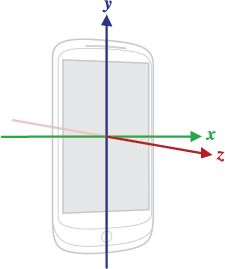
\includegraphics[scale=1]
	{Gambar/axis-device.png}
	\caption{Sumbu Sensor Perangkat Bergerak}
	\label{fig:axis-device}
\end{figure}

Setelah mengetahui sumbu-sumbu sensor perangkat bergerak, langkah selanjutnya adalah menentukan gerakan-gerakan yang dilakukan pada eksperimen ini. Tabel \ref{tab:step-detector-test} menunjukkan gerakan-gerakan yang dilakukan pada perangkat bergerak serta hasil deteksi \textit{step detector sensor}.

\begin{table}[]
    \centering
    \caption{Hasil Eksperimen Pengujian \textit{Step Detector Sensor}}
    \begin{tabular}{|p{1cm}||p{4cm}|p{4cm}|}
    \hline
       No  & Gerakan & Hasil (terdeteksi atau tidak) \\
    \hline
        1 &  Satu kali bergerak pada sumbu $x$ & Tidak terdeteksi \\
    \hline
        2 &  Satu kali bergerak sepanjang sumbu $y$ & Tidak terdeteksi \\
    \hline
        3 &  Satu kali bergerak pada sumbu $z$ & Tidak terdeteksi\\
    \hline
    	4 &  Gerakan sana ke mari pada sumbu $x$ & Terdeteksi\\
    \hline
    	5 &  Gerakan sana ke mari pada sumbu $y$ & Terdeteksi\\
    \hline
    	6 &  Gerakan sana ke mari pada sumbu $z$ & Terdeteksi\\
    \hline
    \end{tabular}
    \label{tab:step-detector-test}
\end{table}

Listing \ref{stepdetectortest} menunjukkan \textit{log} dari aplikasi perangkat bergerak pengujian \textit{step detector sensor} ketika \textit{step detector sensor} mendeteksi rangsang. 

\begin{lstlisting}[language=C,frame=single,caption=\textit{Log console} Pengujian Sensor \textit{Step Detector} Ketika Mendeteksi Langkah Kaki,label=stepdetectortest]
...3985-3985/com.example.stepdetectorsensor D/Step: Step Taken 
...3985-3985/com.example.stepdetectorsensor D/Step: Step Taken 
...3985-3985/com.example.stepdetectorsensor D/Step: Step Taken 
...3985-3985/com.example.stepdetectorsensor D/Step: Step Taken 
...3985-3985/com.example.stepdetectorsensor D/Step: Step Taken
...3985-3985/com.example.stepdetectorsensor D/Step: Step Taken

\end{lstlisting}

Dari eksperimen, dapat disimpulkan bahwa gerakan perangkat ke sana dan ke mari (gerakan vibrasi) adalah gerakan yang memberikan rangsang pada \textit{step detector sensor} sehingga memicu aksi pada aplikasi perangkat bergerak.

\subsection{Cara Memanfaatkan \textit{Step Detector Sensor}}
Untuk membuat animasi atau perubahan pemandangan sesuai rute tempuh yang sudah diperoleh, harus ada perubahan gambar sesuai langkah kaki yang diambil pengguna. Jadi, setiap kali sensor mendapat rangsang, \textit{event} yang dipicu agar terjadi adalah gambar berubah seperti yang dijelaskan pada Subbab \ref{subs:directions-attr-use}, tetapi perubahan gambar \textit{StreetView} yang sesuai \textit{Directions API} harus berubah dengan tahap yang benar agar animasi pemandangan terlihat baik sesuai dengan rute. 